\chapter{Implementation}
In this chapter we describe the implementation of Giflang and provide insights into the decisions we made along the way. As Figure \ref{fig:chap4:overview} shows,
the project consists of two major parts: an interpreter and a~web IDE. It also outlines the API of the interpreter that allows the web IDE to execute programs.
Additionally, there is a~lightweight HTTP server that only serves static files and a~BaaS service for storing user programs.
\begin{figure}[!hbt]
    \centering
    \tikzset{every picture/.style={line width=0.75pt}} %set default line width to 0.75pt        
    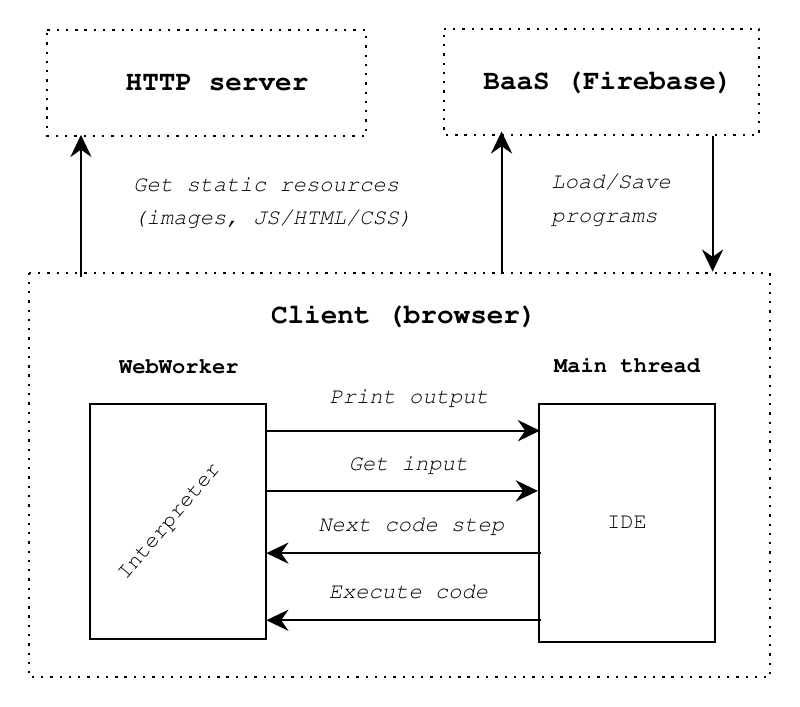
\begin{tikzpicture}[x=0.75pt,y=0.75pt,yscale=-1,xscale=1]
    %uncomment if require: \path (0,461); %set diagram left start at 0, and has height of 461

    %Shape: Rectangle [id:dp6305366313237857] 
    \draw   (102.67,227) -- (187.5,227) -- (187.5,340.33) -- (102.67,340.33) -- cycle ;
    %Shape: Rectangle [id:dp2977546195918692] 
    \draw   (319,227) -- (403.5,227) -- (403.5,341.67) -- (319,341.67) -- cycle ;
    %Straight Lines [id:da951249052099123] 
    \draw    (319.67,299) -- (190.5,299) ;
    \draw [shift={(187.5,299)}, rotate = 360] [fill={rgb, 255:red, 0; green, 0; blue, 0 }  ][line width=0.08]  [draw opacity=0] (10.72,-5.15) -- (0,0) -- (10.72,5.15) -- (7.12,0) -- cycle    ;

    %Straight Lines [id:da5209602217060021] 
    \draw    (319.67,331.33) -- (190.5,331.33) ;
    \draw [shift={(187.5,331.33)}, rotate = 360] [fill={rgb, 255:red, 0; green, 0; blue, 0 }  ][line width=0.08]  [draw opacity=0] (10.72,-5.15) -- (0,0) -- (10.72,5.15) -- (7.12,0) -- cycle    ;

    %Straight Lines [id:da5690847035446265] 
    \draw    (187,269) -- (315.33,269) ;
    \draw [shift={(318.33,269)}, rotate = 180] [fill={rgb, 255:red, 0; green, 0; blue, 0 }  ][line width=0.08]  [draw opacity=0] (10.72,-5.15) -- (0,0) -- (10.72,5.15) -- (7.12,0) -- cycle    ;

    %Shape: Rectangle [id:dp07985742970290266] 
    \draw  [dash pattern={on 0.84pt off 2.51pt}] (73,164.17) -- (430.33,164.17) -- (430.33,358.83) -- (73,358.83) -- cycle ;
    %Shape: Rectangle [id:dp6103195242603674] 
    \draw  [dash pattern={on 0.84pt off 2.51pt}] (82,47) -- (235.5,47) -- (235.5,98) -- (82,98) -- cycle ;
    %Straight Lines [id:da14268622161668265] 
    \draw    (98.17,166) -- (98.17,100.5) ;
    \draw [shift={(98.17,97.5)}, rotate = 450] [fill={rgb, 255:red, 0; green, 0; blue, 0 }  ][line width=0.08]  [draw opacity=0] (10.72,-5.15) -- (0,0) -- (10.72,5.15) -- (7.12,0) -- cycle    ;

    %Straight Lines [id:da3579088417499019] 
    \draw    (188,240) -- (316.33,240) ;
    \draw [shift={(319.33,240)}, rotate = 180] [fill={rgb, 255:red, 0; green, 0; blue, 0 }  ][line width=0.08]  [draw opacity=0] (10.72,-5.15) -- (0,0) -- (10.72,5.15) -- (7.12,0) -- cycle    ;

    %Shape: Rectangle [id:dp03039338044969564] 
    \draw  [dash pattern={on 0.84pt off 2.51pt}] (273,46.33) -- (425,46.33) -- (425,97.33) -- (273,97.33) -- cycle ;
    %Straight Lines [id:da6622259233347125] 
    \draw    (300.83,164.33) -- (300.83,98.83) ;
    \draw [shift={(300.83,95.83)}, rotate = 450] [fill={rgb, 255:red, 0; green, 0; blue, 0 }  ][line width=0.08]  [draw opacity=0] (10.72,-5.15) -- (0,0) -- (10.72,5.15) -- (7.12,0) -- cycle    ;

    %Straight Lines [id:da628472813666374] 
    \draw    (402.5,98) -- (402.5,160.33) ;
    \draw [shift={(402.5,163.33)}, rotate = 270] [fill={rgb, 255:red, 0; green, 0; blue, 0 }  ][line width=0.08]  [draw opacity=0] (10.72,-5.15) -- (0,0) -- (10.72,5.15) -- (7.12,0) -- cycle    ;


    % Text Node
    \draw (256.33,224) node   [align=left] {\textit{{\fontfamily{pcr}\selectfont {\footnotesize Print output}}}};
    % Text Node
    \draw (256,256.33) node   [align=left] {\textit{{\fontfamily{pcr}\selectfont {\footnotesize Get input}}}};
    % Text Node
    \draw (257.33,286) node   [align=left] {\textit{{\fontfamily{pcr}\selectfont {\footnotesize Next code step}}}};
    % Text Node
    \draw (256,317.33) node   [align=left] {\textit{{\fontfamily{pcr}\selectfont {\footnotesize Execute code}}}};
    % Text Node
    \draw (141,284) node  [rotate=-310.46] [align=left] {{\fontfamily{pcr}\selectfont {\footnotesize Interpreter}}};
    % Text Node
    \draw (361.25,284.33) node   [align=left] {{\fontfamily{pcr}\selectfont {\footnotesize IDE}}};
    % Text Node
    \draw (145.33,209.33) node   [align=left] {{\fontfamily{pcr}\selectfont {\footnotesize \textbf{WebWorker}}}};
    % Text Node
    \draw (361.33,208.67) node   [align=left] {{\fontfamily{pcr}\selectfont {\footnotesize \textbf{Main thread}}}};
    % Text Node
    \draw (163.75,72.5) node   [align=left] {{\fontfamily{pcr}\selectfont \textbf{HTTP server}}};
    % Text Node
    \draw (190.67,130) node   [align=left] {{\fontfamily{pcr}\selectfont {\footnotesize \textit{Get static resources}}}\\{\fontfamily{pcr}\selectfont {\footnotesize \textit{(images, JS/HTML/CSS)}}}};
    % Text Node
    \draw (352.08,71.83) node   [align=left] {{\fontfamily{pcr}\selectfont \textbf{BaaS (Firebase)}}};
    % Text Node
    \draw (353.67,129) node   [align=left] {{\fontfamily{pcr}\selectfont {\footnotesize \textit{Load/Save}}}\\{\fontfamily{pcr}\selectfont {\footnotesize \textit{programs}}}};
    % Text Node
    \draw (253.75,184.5) node   [align=left] {{\fontfamily{pcr}\selectfont \textbf{Client (browser)}}};
    \end{tikzpicture}
    \caption{A high-level diagram of the implementation}
    \label{fig:chap4:overview}
\end{figure}

\section{Interpreter}
Every interpreter first \emph{parses} source code and then \emph{executes} the parsed tree (Fig \ref{fig:chap4:interpreter}). There is a~room for a~lot of optimizations along the way in order
to make the execution as fast as possible. However, we do not incorporate any optimizations into the interpreter and only execute the parsed tree node by node.

\begin{figure}[!hbt]
    \centering
    \tikzset{every picture/.style={line width=0.75pt}} %set default line width to 0.75pt        

    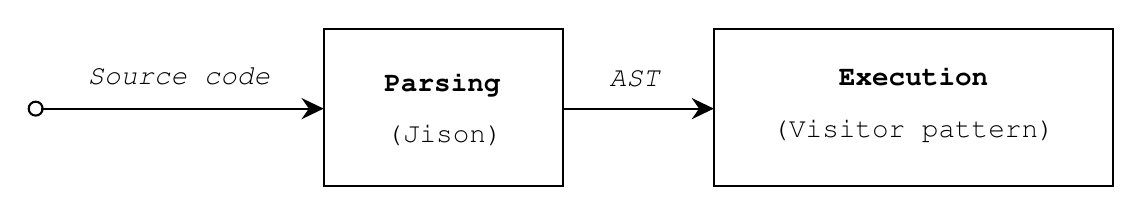
\begin{tikzpicture}[x=0.75pt,y=0.75pt,yscale=-1,xscale=1]
    %uncomment if require: \path (0,622); %set diagram left start at 0, and has height of 622

    %Shape: Rectangle [id:dp28122229657926034] 
    \draw   (226.5,34) -- (341.5,34) -- (341.5,110) -- (226.5,110) -- cycle ;
    %Straight Lines [id:da9888936135364137] 
    \draw    (411.25,72.5) -- (341.5,72.5) ;

    \draw [shift={(414.25,72.5)}, rotate = 180] [fill={rgb, 255:red, 0; green, 0; blue, 0 }  ][line width=0.08]  [draw opacity=0] (10.72,-5.15) -- (0,0) -- (10.72,5.15) -- (7.12,0) -- cycle    ;
    %Shape: Rectangle [id:dp7793277711435098] 
    \draw   (414.5,34) -- (606.5,34) -- (606.5,110) -- (414.5,110) -- cycle ;
    %Straight Lines [id:da7940866772557511] 
    \draw    (223.25,72.5) -- (89.85,72.5) ;
    \draw [shift={(87.5,72.5)}, rotate = 180] [color={rgb, 255:red, 0; green, 0; blue, 0 }  ][line width=0.75]      (0, 0) circle [x radius= 3.35, y radius= 3.35]   ;
    \draw [shift={(226.25,72.5)}, rotate = 180] [fill={rgb, 255:red, 0; green, 0; blue, 0 }  ][line width=0.08]  [draw opacity=0] (10.72,-5.15) -- (0,0) -- (10.72,5.15) -- (7.12,0) -- cycle    ;

    % Text Node
    \draw (283.5,61) node   [align=left] {{\fontfamily{pcr}\selectfont \textbf{Parsing}}};
    % Text Node
    \draw (510.5,57) node   [align=left] {{\fontfamily{pcr}\selectfont \textbf{Execution}}};
    % Text Node
    \draw (376.5,58) node   [align=left] {{\fontfamily{pcr}\selectfont \textit{AST}}};
    % Text Node
    \draw (284.5,85) node   [align=left] {{\fontfamily{pcr}\selectfont (Jison)}};
    % Text Node
    \draw (510.5,83) node   [align=left] {{\fontfamily{pcr}\selectfont (Visitor pattern)}};
    % Text Node
    \draw (156.5,57) node   [align=left] {{\fontfamily{pcr}\selectfont \textit{Source code}}};
    \end{tikzpicture}
    \caption{A diagram of the Giflang interpreter}
    \label{fig:chap4:interpreter}
\end{figure}

\subsection{Parsing}
Parser is an interpreter component that checks whether the input source conforms to the rules of the formal grammar of a~language. Additionally, parsers help
building an AST from the source code. In the very beginning of this thesis we briefly explained what grammar rules and ASTs are
(Fig \ref{fig:chap1:tokens_and_grammar}).

Parsers usually consist of two separate parts: \emph{lexing} or \emph{tokenization} and \emph{parsing}. A lexer splits input text into \emph{tokens}.
For example it can split an input \texttt{'4 + size'} into following tokens:
\begin{code}
// Sample tokens for an input '4 + size'
[{ "Type": "NUMBER", "Text": "4" },
 { "Type": "OPERATOR", "Text": "+" },
 { "Type": "IDENTIFIER", "Text": "size" }]
\end{code}

Grammar rules are then defined in terms of tokens, for example:
\begin{figure}[!hbt]
\begin{code}
expression -> factor OPERATOR expression
expression -> factor
factor -> IDENTIFIER
factor -> NUMBER
\end{code}
    \caption{An example of a~grammar definition}
    \label{fig:chap4:grammar}
\end{figure}

The grammar above defines a~language consisting of expressions that can contain numbers and identifiers. It is very minimal as it does not account
for operator precedence or parenthesis. Lowercase words are nonterminals and capitalized words are terminals. \emph{Terminal symbols} are elementary
symbols and can not be replaced by other terminals or nonterminals. \emph{Nonterminals} can appear on the left side of productions and they are replaced by groups
of terminal symbols according to the production rules.

In order to parse a~grammar like the one above, we can either create our own parser or use \emph{a parser generator}. We will briefly describe both options.
There are many ways of creating a~custom parser, but we will discuss the most common one, a~recursive-descent parser. Parsers are a~large topic and
we do not intent to dive deep into it.

\subsubsection*{Recursive-descent parser}
A recursive-descent parser is a~method of creating a~parser using mutually recursive procedures where each procedure implements one of the nonterminals
of the grammar. To give us a~better idea of what it means to create a~function for each nonterminal, we created a~parser for the grammar from Figure
\ref{fig:chap4:grammar} in Python.
\begin{code}
# Unimplemented functions:
#   * curToken -- returns the current token
#   * curTokenText -- returns the current token's text
#   * nextToken -- advances to the next token

def factor():
    if curToken() == 'IDENTIFIER':
        # action1(curTokenText())
        nextToken()
    elif curToken() == 'NUMBER':
        # action2(curTokenText())
        nextToken() 
    else:
        raise Exception("factor: syntax error")

def expression():
    factor()
    if curToken() == 'OPERATOR':
        nextToken()
        expression()
        # action3(curTokenText())
        return

    # action4(curTokenText())
\end{code}

We can see that the grammar can be transformed into the code very naturally using a~recursive-descent parser. The \texttt{'\# actionX(curTokenText())'} comments
mark places where grammar rules are applied and we could add bits of code there that would build a~derivation tree.

Recursive-descent parsers can run in a~linear time with respect to the input string size, granted that the parsed grammar is an LL(k) \cite{aho_sethi_ullman_2002}.
\emph{An LL(k) grammar} is a~context-free grammar that is parsed by an LL parser \cite{aho_sethi_ullman_2002}, which parses the input from \textbf{L}eft
to right and creates a~\textbf{L}eftmost derivation. Additionally, it requires at most $k$ lookahead tokens to uniquely identify which rule should be applied next.

\subsubsection*{Parser generators}
Creating parsers can be a~repetitive process -- applying the same patterns to different grammars. Parser generators solve this by generating parsers from grammar
specifications. There are dozens of parser generators, but we will only describe one of them, GNU Bison \cite{Bison}

We will also use Flex in the examples, a~lexical analyzer generator that is often used alongside Bison. Both Flex and Bison can target C, C++, and Java.

Flex takes token descriptions as regular expressions. The following code is not a~valid Flex source, but it demonstrates the idea behind Flex:
\begin{code}
%{ %}

DIGIT           [0-9]
LETTER          [a-zA-Z]

%%
{DIGIT}+                        return NUMBER;
{LETTER}({LETTER}|{DIGIT})*     return IDENTIFIER;
[+-]                            return OPERATOR;
%%
\end{code}

Flex can create a~lexer from the source code above. Let us now show a~Bison source for the grammar from Figure \ref{fig:chap4:grammar}.
\newpage
\begin{code}
%{ %}

%token NUMBER IDENTIFIER OPERATOR
%start expression

%%
expression
    : factor OPERATOR expression    { /* Action */ }
    | factor                        { /* Action */ }
    ;
factor
    : IDENTIFIER                    { /* Action */ }
    | NUMBER                        { /* Action */ }
    ;
%%
\end{code}

Parser generators can employ many different parsing algorithms, but the most common ones are LL parser and LALR(1) \cite{aho_sethi_ullman_2002}, as it is also
case with Bison. We will not describe the mentioned parsers since we do not find it important in our case.

\subsubsection*{Conclusion}
The main advantage of creating a~custom parser over a~parser generator is the option to create better error reporting and error recovery. It would also be a
good learning experience to make a~parser with a~lexer from scratch. However, we opted for using a~parser generator as in the very beginning of the project
we wanted to focus on interpreting the AST rather than parsing.

There are numerous parser generators for JavaScript, most notably ANTLR \cite{ANTLR} and acorn \cite{acorn}. Since we had prior experience with Bison, we
decided to use Jison \cite{Jison}, a~Bison-like JavaScript library. Our Jison grammar is defined at \texttt{interpreter/ast/giflang.jison}.

\subsection{Employing the Visitor pattern}
Probably the easiest way to create an interpreter is by using \emph{the interpreter design pattern}. The basic idea is to have a~class for each symbol
(terminal or nonterminal). The syntax tree is then build from these classes. Every class defines an \texttt{evaluate} method that interprets given node
of the syntax tree, possibly evaluating its child nodes as well.

Below is a~Python example of the interpreter pattern that evaluates the grammar from Figure \ref{fig:chap4:grammar}. We did not define a~class for each
symbol to make it more concise.
\begin{code}
class Node:
    def evaluate(self, env):
        raise Exception('Method not implemented')

class Expression(Node):
    def __init__(self, left, right, op):
        self.left, self.right, self.op = left, right, op

    def evaluate(self, env):
        lval, rval = self.left.evaluate(env), self.right.evaluate(env)
        if self.op == '+':
            return lval + rval
        elif self.op == '-':
            return lval - rval
        else:
            raise Error('Unknown operator ' + self.op)

class Number(Node):
    def __init__(self, value):
        self.value = value
    
    def evaluate(self, env):
        return self.value

class VariableAccess(Node):
    def __init__(self, identifier):
        self.identifier = identifier
    
    def evaluate(self, env):
        if self.identifier in env:
            return env[self.identifier]
        else:
            raise Error('Unknown variable ' + self.identifier)

# Expression: 2 + x - 9
exp = Expression(
    Number(2),
    Expression(VariableAccess('x'), Number(9), '-'),
    '+')
# Prints 3
print(exp.evaluate({'x': 10}))
\end{code}

When using the interpreter pattern, the execution logic in the form of \texttt{evalute} methods is spread among multiple classes. In order to couple the
logic together we decided to use the visitor pattern. \emph{The visitor design pattern} is a~way of separating an algorithm from an object structure on
which it operates. In this case it separates the \texttt{evaluate} methods from the AST node definitions.
\begin{code}
class Node:
    def accept(self, visitor):
        raise Exception('Method not implemented')

class Expression(Node):
    def __init__(self, left, right, op):
        self.left, self.right, self.op = left, right, op

    def accept(self, visitor):
        return visitor.visitExpression(self)

# We omit implementation of Number and VariableAccess nodes as
# they are very similar to the Expression node, i.e., they only
# define an accept method.

class Interpreter:
    def __init__(self, env):
        self.env = env
    
    def visitExpression(self, exprNode):
        lval = exprNode.left.accept(self)
        rval = exprNode.right.accept(self)
        if exprNode.op == '+':
            return lval + rval
        elif exprNode.op == '-':
            return lval - rval
        else:
            raise Error('Unknown operator ' + exprNode.op)
    
    def visitNumber(self, numberNode):
        return numberNode.value
    
    def visitVariableAccess(self, variableAccessNode):
        id = variableAccessNode.identifier
        if id in self.env:
            return self.env[id]
        else:
            raise Error('Unknown variable ' + id)

# Expression: 2 + x - 9
exp = Expression(
    Number(2),
    Expression(VariableAccess('x'), Number(9), '-'),
    '+')
interpreter = Interpreter({'x': 10})
# Prints 3
print(exp.accept(interpreter))
\end{code}

In the example above, the Interpreter class is a~Visitor and its methods implement the execution logic.

The types of return values of different nodes might be different. When implementing the interpreter we found three different return types:
\begin{enumerate}
    \item \emph{An instance} -- for example literal or expression nodes return an instance
    \item \emph{An instance reference} -- accesing a~variable, a~property, or an array element has to result in an assignable value (i.e., a~reference)
    \item \emph{A completion} -- cycles can contain \texttt{break} or \texttt{continue} statements that do not result in an instance, but rather a~completion
        that carries information about how a node finished its execution, i.e., normally, with a \texttt{break}, \texttt{continue} or a \texttt{return}
\end{enumerate} 

In the implementation, we split the nodes into three categories based on their return types: \texttt{ValueExpr}, \texttt{RefExpr}, and \texttt{Stmt}.
The node classes can be found in \texttt{interpreter/ast/\{expr, stmt\}.ts} files and the interpreter visitor in \texttt{interpreter/interpreter.ts}. 

\subsection{Class hierarchy of the object model}
In Section \ref{chap3:object_model} we outlined the object model of Giflang. In order to implement it in a~statically-typed language like TypeScript, we
need to define a~class hierarchy that will represent the object model. Since everything is an object, everything has to derive from a~single class. We named
this class \texttt{Instance}.
\begin{figure}[!hbt]
	\includegraphics[width=1\textwidth]{../img/class_hierarchy}
    \caption{Class hierarchy of the object model}
	\label{fig:chap4:class_hierarchy}
\end{figure}

Classes \texttt{Instance} and \texttt{Class} are \emph{abstract}. As we can see from Figure \ref{fig:chap4:class_hierarchy}, classes have their
respective instance classes; for example there is \texttt{NumberClass} and \texttt{NumberInstance}. This results in creating a~relatively big number
of classes, but we did not find any other suitable model, because different classes of instances need to hold different value types. To illustrate this,
a \texttt{Number} needs to hold a~number as its value, while \texttt{String} needs to hold a~string, etc.

We could create a~templated \texttt{Instance<T>} class that would have a~\texttt{value: T} property. This way, we would be able to reduce the number of
classes. However, some of the instance classes also incorporate additional functionality, e.g., \texttt{UserFunctionInstance} implements a~\texttt{call} method
that allows calling the function. Since there are more cases like this one, we decided to create all instances in a~uniform fashion and did not opt for the
generic \texttt{Instance<T>} approach.

Classes define their methods as static functions and during their initialization these methods are assigned to the class objects they represent.
A code snippet below demonstrates this:
\begin{code}
class NumberClass extends Class {
    // Overloads '+' operation of two numbers.
    static __add__(
        args: Instance[],
    ): NumberInstance {
        CheckArity(args, /* expectedArity = */ 2)
        const lhs = args[0].castOrThrow(NumberInstance)
        const rhs = args[1].castOrThrow(NumberInstance)
        return new NumberInstance(
            /* klass = */ NumberClass.get(), lhs + rhs)
    }

    constructor() {
        this.fields.set(
            /* fieldName = */ '__add__',
            new WrappedFunctionInstance(
                /* klass = */ WrappedFunctionClass.get(),
                NumberClass.__add__,
                /* functionName = */ '__add__'
            )
        )
    }
}
\end{code}

Since \texttt{NumberClass.\_\_add\_\_} is a~TypeScript function it needs to be wrapped around Giflang's object. We named this wrapper a~\texttt{WrappedFunctionInstance}.
The code in the actual implementation is a~little more abstract since repeating this for every operation would need a~lot of boilerplate.

When writing the code, we often needed the class objects, usually for instantiation, e.g.,
\texttt{new NumberInstance(NumberClass.get(), lhs + rhs)} in the code example above. In this case, \texttt{NumberClass.get()} is a~\texttt{NumberClass} instance. Since only one
instance of each class object is needed, we used \emph{the singleton pattern}. In hindsight, it was not the best choice, because it allows changing
the interpreter state in between multiple invocations.
\begin{code}
const interpreter1 = new Interpreter()
// This code can change state of the singletons, for example
// override __add__ operation on the NumberClass.
interpreter1.visitProgramStmt(ParseGiflang('"evil" source code'))

const interpreter2 = new Interpreter()
// The second interpreter uses the same singletons and hence
// their state will be changed.
interpreter2.visitProgramStmt(ParseGiflang('source code'))
\end{code}

However, since we spawn a~new WebWorker with each code run, this was not an issue. If we decide to reuse the same WebWorker, we can use a~global registry
instead of singletons. Class objects in the registry can then be reinstantiated after each code execution.

\subsection{Environments}
The bindings that associate variables to values need to be stored somewhere. The data structure that holds these bindings is called an \emph{``environment''}.
It is basically a~\emph{map} where the keys are variable names and the values are the variable’s values. The environment also needs to store a~reference
to an enclosing environment, in order to support variable shadowing. To illustrate this, we show a~JavaScript code snippet with a~nested block.
\begin{code}
let x = 'global'
{
    let x = 'local'
}
\end{code}
Inside the block enclosed with curly braces is a~definition of a~variable with the same name, \texttt{x}, as the one in the global scope. The inner \texttt{x}
\emph{shadows} the outer \texttt{x}. The environment right after the creation of the inner variable with the text \texttt{'local'} is shown in Figure
\ref{fig:chap4:environment}.

\begin{figure}[!hbt]
    \centering
    \tikzset{every picture/.style={line width=0.75pt}} %set default line width to 0.75pt        

    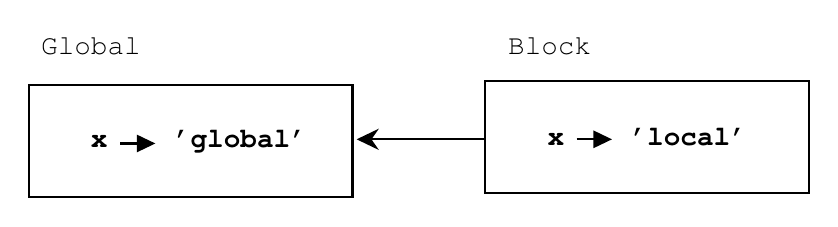
\begin{tikzpicture}[x=0.75pt,y=0.75pt,yscale=-1,xscale=1]
    %uncomment if require: \path (0,622); %set diagram left start at 0, and has height of 622

    %Shape: Rectangle [id:dp28122229657926034] 
    \draw   (115.5,36) -- (271.5,36) -- (271.5,90) -- (115.5,90) -- cycle ;
    %Straight Lines [id:da4197097698317285] 
    \draw    (335.5,62) -- (276.5,62) ;
    \draw [shift={(273.5,62)}, rotate = 360] [fill={rgb, 255:red, 0; green, 0; blue, 0 }  ][line width=0.08]  [draw opacity=0] (10.72,-5.15) -- (0,0) -- (10.72,5.15) -- (7.12,0) -- cycle    ;

    %Straight Lines [id:da14520356555697966] 
    \draw    (159.5,64) -- (173.5,64) ;
    \draw [shift={(176.5,64)}, rotate = 180] [fill={rgb, 255:red, 0; green, 0; blue, 0 }  ][line width=0.08]  [draw opacity=0] (8.93,-4.29) -- (0,0) -- (8.93,4.29) -- cycle    ;

    %Shape: Rectangle [id:dp8897420928474284] 
    \draw   (335.5,34) -- (491.5,34) -- (491.5,88) -- (335.5,88) -- cycle ;
    %Straight Lines [id:da6354911803773373] 
    \draw    (379.5,62) -- (393.5,62) ;
    \draw [shift={(396.5,62)}, rotate = 180] [fill={rgb, 255:red, 0; green, 0; blue, 0 }  ][line width=0.08]  [draw opacity=0] (8.93,-4.29) -- (0,0) -- (8.93,4.29) -- cycle    ;


    % Text Node
    \draw (145.5,17) node   [align=left] {{\fontfamily{pcr}\selectfont Global}};
    % Text Node
    \draw (197.5,62.87) node   [align=left] {{\fontfamily{pcr}\selectfont \textbf{x \ \ \ 'global'}}};
    % Text Node
    \draw (366.5,17) node   [align=left] {{\fontfamily{pcr}\selectfont Block}};
    % Text Node
    \draw (413.5,60.87) node   [align=left] {{\fontfamily{pcr}\selectfont \textbf{x \ \ \ 'local'}}};
    \end{tikzpicture}

    \caption{An example of a~nested environment}
	\label{fig:chap4:environment}
\end{figure}

We decided to use the native \texttt{Map} implementation of JavaSript in the interpreter. The standard \texttt{Map} is a~mutable data structure. This means
that environments captured by a~closure might change outside of the closure function.
\begin{code}
$f$ F(){
    G = $f$(){ $\lambda$(Z); };
    Z = 8;
    G();
}
# Prints 8
F();
\end{code}
The code above is a~Giflang source code, note that \texttt{$\lambda$} is a~print function. The closure which prints variable \texttt{Z} is created on
the second line, but at the time of its creation \texttt{Z} does not exist. Therefore, we might expect that invoking \texttt{G} fails.
However, it is not the case with mutable environments as the name resolution of free variables occurs at closure execution.

The closure captures the environment created for the function \texttt{F}. In the same environment, \texttt{Z} is assigned after the closure definition and hence
when \texttt{G} is invoked, \texttt{Z} exists inside the closure.

To resolve free variables occurs at closure creation, we could use a~persistent data structure. A \emph{persistent data structure} can never be directly modified. Instead, any ``modification''
to an existing structure produces a~brand new object that contains all of the original data and the new modification. The original is left unchanged.

By using a~Persistent Map data structure we could create a~persistent environment, i.e., an environment where any addition of a~variable would create 
a new environment. This would require another layer of indirection in the map values, because multiple maps of different environments could contain the same
variable. Changing the variable's value in one environment should change it in all others as well.

We decided to stick with mutable environments because we believe that use of closures that leads to the issue described above is rare. Moreover, this behavior
is consistent with both Python and JavaScript.

\subsection{Code-stepping (debugger)}
In order to support code-stepping, we need to be able to pause the execution at certain AST nodes and resume it until another AST node that stops the execution
is encountered. We illustrate this in the following example.
\begin{code}
class Interpreter {
    //...
    visitAssignmentValueExpr(expr: AssignmentValueExpr): Instance {
        const l = this.evaluateRef(expr.lhs)
        const r = this.evaluate(expr.rhs)
        this.waitForNextStep()
        l.set(r)
        return r
    }
    //...
}
\end{code}
The above function implements a~standard assignment. It evaluates left-hand side to a~reference, right-hand side to a~value, assigns the value to the
referenced variable, and returns the value. Additionally, the method \texttt{waitForNextStep} is supposed to pause the execution after the evaluation of 
both sides.

We need a~mechanism of capturing the current state of the interpreter, e.g., call stack and local variables, storing this state, and then resuming the execution
from this state later on. What we described is essentially a~\emph{continuation}.

\subsection*{Continuation-passing style}
\label{chap4:continuations}
Implementing continuations using the continuation-passing style uses two simple rules\footnote{http://matt.might.net/articles/by-example-continuation-passing-style/}:
\begin{itemize}
    \item Procedures are not allowed to explicitly \texttt{return} to their callers
    \item Procedures take a~callback to invoke upon their return value
\end{itemize}
An extra argument is added to every function which is used to pass the function's continuation. This continuation is a~callback
representing actions that must happen after the function ``returns''. The call stack becomes obsolete in continuation-passing style -- when
a function calls another function, it is the last thing it does. Instead of waiting for the called function to return, it puts any work
it wants to do afterwards into a~continuation, which it passes to the function.

The previous example can be written as follows.
\newpage
\begin{code}
class Interpreter {
    //...
    visitAssignmentValueExpr(
        expr: AssignmentValueExpr, c: Continuation) {
        this.evaluateRef(expr.lhs, (lres: ValueRef) => {
            this.evaluate(expr.rhs, (rres: Instance) => {
                this.waitForNextStep(
                    () => {
                        lres.set(rres)
                        c(rres)
                })
            })
        })
    }
    waitForNextStep(c: Continuation) {
        document.getElementById('button').addEventListener(
            "click",
            c
        );
    }
    //...
}
\end{code}

On every function call, a~continuation with the rest of the function code is passed. Finally, \texttt{waitForNextStep} uses its continuation as the \texttt{Button}'s
\texttt{onClick} callback. In our case, we would need to employ a~few more tricks as we want to run the interpreter in a~separate WebWorker, but the idea
outlined here could still be used.

The disadvantage of continuation-passing style is that in order to work efficiently, without overpopulating the call stack, the language should support the tail
call optimization. The \emph{tail call optimization} (TCO) allows procedure calls in tail position to be implemented as efficiently as goto statements, instead of adding
a new stack frame onto the call stack. Even though JavaScript ES6 standard explicitly requires TCO, as of January 1st, 2020, only Safari supports it.

There is also another way of bringing continuations to JavaScript described in the article \emph{Exceptional Continuations in JavaScript}
\cite{ExceptionalContinuations} that does not have the performance issues mentioned above. The authors propose splitting every function into
multiple states and record which state is currently being executed. Once a~\texttt{suspend} function is called, an exception is thrown. As
the call stack unwinds, every function catches the exception, records its state in the exception object and rethrows it. The exception object
now holds the state and it is essentially a~continuation. A \texttt{resume} function takes the ``exceptional continuation'' created earlier and restores the state.

\subsection*{Async/await and generators}
Another way of implementing the code-stepping is using promises. A \emph{Promise} is a~proxy for a~value not necessarily known when the promise is created.
It allows associating handlers with an asynchronous action's eventual success value or failure reason. JavaScript also supports \emph{async/await} to
ease working with promises.
\begin{code}
class Interpreter {
    //...
    async visitAssignmentValueExpr(expr: AssignmentValueExpr)
        : Promise<Instance> {
        const l = await this.evaluateRef(expr.lhs)
        const r = await this.evaluate(expr.rhs)
        await this.waitForNextStep()
        l.set(r)
        return r
    }
    async waitForNextStep(c: Continuation) {
        let outsideResolve
        const retPromise = new Promise((resolve) => { 
            outsideResolve = resolve; 
        })
        document.getElementById('button').addEventListener(
            "click",
            outsideResolve
        )
        return retPromise
    }
    //...
}
\end{code}
In order to resolve the \texttt{retPromise} returned from the \texttt{waitForNextStep} method only after the button is clicked, we store the promise's resolve
function outside of the promise.

Another option is to use \emph{generator functions}, an ES6 addition that allows \texttt{yield}ing from a~function and resuming it later. However, both generators
and async/await require propagation of generators and async/await through the whole interpreter codebase. There is no way of synchronously waiting for a~promise
in JavaScript as opposed to for example \texttt{promise.wait()} in C\#.
 
\subsection*{Atomics API}
\label{chap4:atomics}
In order to allow sharing memory between WebWorkers and the main thread, \texttt{SharedArrayBuffer}s were introduced. This construct allows us to create
views on shared, typed memory. Rather than copying data from the main thread to the Worker and back again, we can update the same shared memory from both sides.

Being able to update data from multiple threads might introduce race conditions and other synchronization issues. The \emph{Atomics API} addresses that by providing
the basic means of synchronization.

We can leverage these technologies to implement code-stepping. Our approach below sets the first (and only) element of the buffer \texttt{flag} to $0$ in a~WebWorker
and waits until its value is changed. The main thread sets the \texttt{flag} to $1$ when a~button is clicked.
\newpage
\begin{code}
// WebWorker
const sab = new SharedArrayBuffer(4)
const flag = new Int32Array(this.sab)

class Interpreter {
    waitForNextStep() {
        // Set the flag to 0 and wait until it changes
        Atomics.store(flag, 0, 0)
        Atomics.wait(flag, 0, 0)
    }
}

// Main thread
document.getElementById('button').addEventListener(
    "click",
    () => {
        Atomics.store(this.flag, 0, 1)
        Atomics.notify(this.flag, 0, 1)
    })
)
\end{code}
For simplicity, the example does not deal with sharing the buffer \texttt{flag} between the worker and the main thread.

Atomics and SharedArrayBuffers were well supported by all major browsers, but due to the \emph{timing attacks} (Meltdown and Spectre) they were disabled on
January 5th, 2018. Chrome has re-enabled it from the version $68$ and Firefox supports it under a~flag from the version $57$. At the time of
writing this thesis\footnote{December 26th, 2019}, discussions at the ECMAScript's official GitHub repository suggest that SharedArrayBuffers and Atomics
will not be removed from the standard in the future and thus the browsers should once again support them.

\subsection*{Iterative traversal of an AST}
Earlier we mentioned JS-Interpreter \cite{JSInterpreter} in Section \ref{chap3:javascript}. It is a~JavaScript interpreter that supports code-stepping, but
it does not use any of the aforementioned methods to implement it. The idea behind JS-Interpreter is to simply traverse the AST iteratively, using an explicit
stack, rather than recursively.

It uses a~stack that stores a path from the root to the current node. Nodes that need to pass values further up the tree, for example expression nodes, can store
the return value in the object right above them in stack, i.e., their parent. Since nodes can have multiple children, they can be in different states
based on how many of the children they already processed.

\begin{code}
const stack = [astRoot]

function stepAssignment(stack) {
    state = stack[stack.length - 1]
    if (!state.doneLeft_) {
        state.doneLeft_ = true
        stack.push(new State(node.left))
        return
    }
    if (!state.doneRight_) {
        state.doneRight_ = true
        stack.push(new State(node.right))
        return
    }
    state.leftReference.set(state.rightValue)
    stack.pop()
    stack[stack.length - 1].value = state.rightValue
    return
}

function next() {
    type = stack[stack.length - 1].type
    if (type === 'assignment') {
        stepAssignment(stack)
    } else if (type === '...') {
        // ...
    }
}
\end{code}

The above code very roughly illustrates the idea. It does not account for scoping and other important details.

\subsection*{Conclusion}
We implemented the interpreter using recursive calls and the visitor pattern, and only after that started incorporating code-stepping into it. We first used
the async/await approach and thus propagated async/await through the whole interpreter. This caused a~very serious slowdown of the execution. Therefore, we ended
up using the Atomics API approach, even though it has a~limited support as of now. We found implementing our own continuations using the continuation-passing style
very verbose and also prone to serious performance issues. The exceptional continuations do not have the performance issues, but come at a~price of even more boilerplate.

In retrospect, iteratively traversing the AST would be the best option because it does not come with any browser compatibility issues. The author of this thesis
will use Giflang at the programming camps with a~full control over the installed software on the machines and hence the compatibility will not be an issue.
However, shall this project be released to the public while not enough browsers brought back the Atomics API, we would refactor the interpreter to
use the method of iteratively traversing the AST.

\section{IDE}
We do not aspire to create a~feature-rich IDE, but rather a~minimal, proof-of-concept IDE. As discussed in Section \ref{chap2:spa}, we decided to use React
for the development of the IDE. We did not find a~way of reusing existing React text editors and decided to create our own.

\subsection{Layout}
IDEs usually share common patterns when it comes to their layouts. Big main editing area, console at the bottom, tree folder view in the sidebar, etc. We decided
to use a~very basic layout as we wanted to keep the main editing area as big as possible, because the images take a~lot of screen space.
\begin{figure}[!hbt]
    \centering
    \tikzset{every picture/.style={line width=0.75pt}} %set default line width to 0.75pt        

    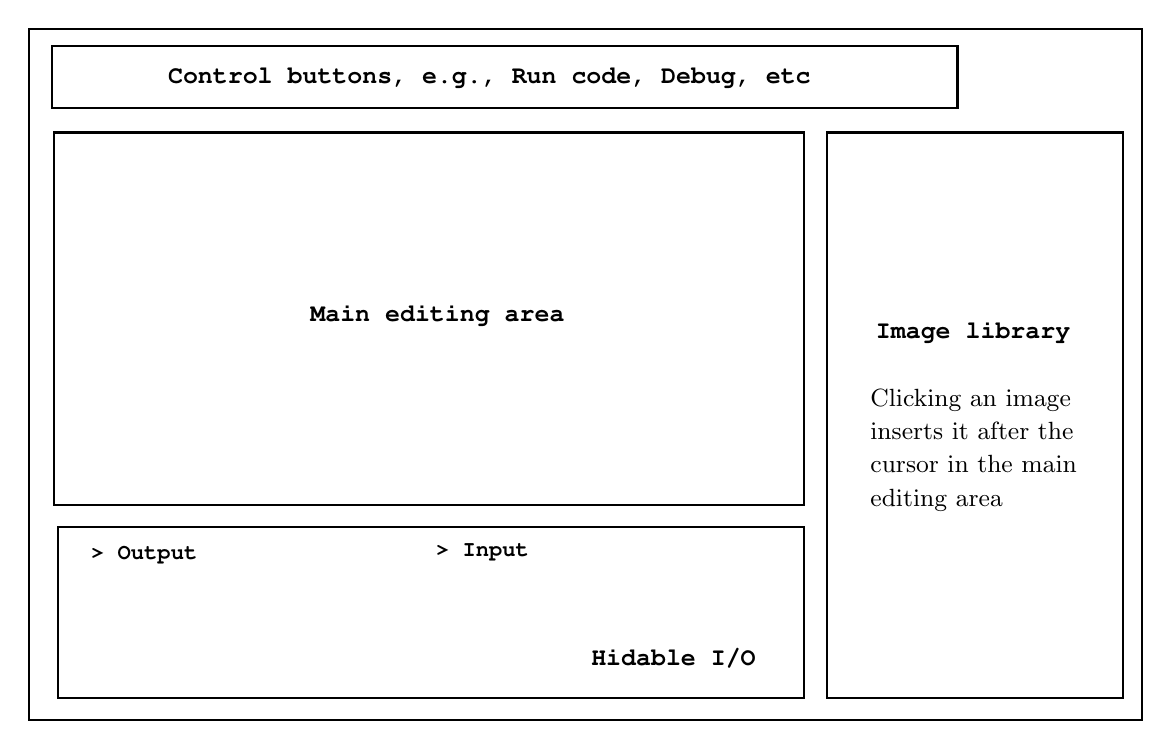
\begin{tikzpicture}[x=0.75pt,y=0.75pt,yscale=-1,xscale=1]
    %uncomment if require: \path (0,622); %set diagram left start at 0, and has height of 622

    %Shape: Rectangle [id:dp11333916049726755] 
    \draw   (59,88) -- (595.5,88) -- (595.5,421) -- (59,421) -- cycle ;
    %Shape: Rectangle [id:dp6658637717016911] 
    \draw   (70.38,96.54) -- (506.5,96.54) -- (506.5,126) -- (70.38,126) -- cycle ;
    %Shape: Rectangle [id:dp9314788663307298] 
    \draw   (71.33,138) -- (432.5,138) -- (432.5,317.59) -- (71.33,317.59) -- cycle ;
    %Shape: Rectangle [id:dp4753802887311882] 
    \draw   (443.5,138) -- (586.01,138) -- (586.01,410.56) -- (443.5,410.56) -- cycle ;
    %Shape: Rectangle [id:dp20916144816663373] 
    \draw   (73.23,328.03) -- (432.5,328.03) -- (432.5,410.56) -- (73.23,410.56) -- cycle ;

    % Text Node
    \draw (255.92,226.04) node   [align=left] {{\fontfamily{pcr}\selectfont \textbf{{\small Main editing area}}}};
    % Text Node
    \draw (280.94,111.35) node   [align=left] {{\fontfamily{pcr}\selectfont \textbf{{\small Control buttons, e.g., Run code, Debug, etc}}}};
    % Text Node
    \draw (369.65,391.29) node   [align=left] {{\fontfamily{pcr}\selectfont \textbf{{\small Hidable I/O}}}};
    % Text Node
    \draw (114.65,341.29) node   [align=left] {{\fontfamily{pcr}\selectfont \textbf{{\footnotesize > Output}}}};
    % Text Node
    \draw (277.65,340.29) node   [align=left] {{\fontfamily{pcr}\selectfont \textbf{{\footnotesize > Input}}}};
    % Text Node
    \draw (514,234) node   [align=left] {\textbf{{\fontfamily{pcr}\selectfont {\small Image library}}}};
    % Text Node
    \draw (514.26,291.05) node   [align=left] {{\small Clicking an image}\\{\small inserts it after the}\\{\small cursor in the main}\\{\small editing area}};
    \end{tikzpicture}
    \caption{The layout of the IDE}
    \label{fig:chap4:layout}
\end{figure}
Figure \ref{fig:chap4:layout} shows our layout. Our IDE is a~\emph{fullscreen web application}, i.e., a~website that can not be scrolled as a~whole, but
its internal components might be scrollable. Creating a~fullscreen web application requires some CSS trickery, but it is much easier nowadays, since Flexboxes
have been widely adopted across browsers.

\subsection{Choosing an animation format}
There are many image formats that support animations. We will briefly describe the ones supported by the most browsers.
\begin{itemize}
    \item \emph{GIF} is the oldest and simplest image format still commonly used on the web. It lacks alpha transparency\footnote{Alpha transparency is a~way to
    support \emph{gradations} of opacity}, has a~limited color pallete of only 256 colors per frame, and has a~relatively large file size.
    Despite all of the cons we mentioned, it remains widely used and supported.

    \item \emph{APNG} is an extension of the PNG. It supports 24-bit images, an 8-bit alpha channel, and offers smaller file sizes compared to GIFs. The APNG format
    is now well supported in all major browsers except for Microsoft Edge.

    \item \emph{WebP} is a~relatively new image format that was created as a~derivative of the VP8 video format. It employs both lossy and lossless compression.
    Compared to lossless compressions of GIF and APNG, lossy compression of WebP allows achieving better file sizes of animations. It is currently supported
    in all major browsers except for Safari and Internet Explorer.
\end{itemize}

Since we need to load a~lot of animations, keeping file sizes small is a~priority and hence we decided to use the WebP format.

\subsection{State management (Redux)}
React is component-based, where a~\emph{component} is a~JavaScript class or function that describes how a~section of the UI should look. 
Every component can have multiple child components. This means that the components together form a~tree. Components can hold data in
two forms:
\begin{itemize}
    \item \emph{Props} -- passed to the component from its parent (similar to function parameters)
    \item \emph{State} -- managed within the component (similar to variables declared within a~function)
\end{itemize}

\emph{Props} should not be mutated because React does not update the UI when props are changed. Only the \emph{state} of a~component can be mutated via a~special
component method \texttt{setState}. We often need to change the state of a~component \texttt{A} from its subcomponent \texttt{B}. In order to do so, we need to wrap
the call of \texttt{A}'s \texttt{setState} and pass this callback along the tree to \texttt{B}. This can be viewed as data flowing down the tree and state changes
flowing up.

\begin{figure}[!hbt]
    \centering
\tikzset{
pattern size/.store in=\mcSize, 
pattern size = 5pt,
pattern thickness/.store in=\mcThickness, 
pattern thickness = 0.3pt,
pattern radius/.store in=\mcRadius, 
pattern radius = 1pt}
\makeatletter
\pgfutil@ifundefined{pgf@pattern@name@_zsxk942iq}{
\pgfdeclarepatternformonly[\mcThickness,\mcSize]{_zsxk942iq}
{\pgfqpoint{0pt}{-\mcThickness}}
{\pgfpoint{\mcSize}{\mcSize}}
{\pgfpoint{\mcSize}{\mcSize}}
{
\pgfsetcolor{\tikz@pattern@color}
\pgfsetlinewidth{\mcThickness}
\pgfpathmoveto{\pgfqpoint{0pt}{\mcSize}}
\pgfpathlineto{\pgfpoint{\mcSize+\mcThickness}{-\mcThickness}}
\pgfusepath{stroke}
}}
\makeatother
\tikzset{every picture/.style={line width=0.75pt}} %set default line width to 0.75pt        

\begin{tikzpicture}[x=0.75pt,y=0.75pt,yscale=-1,xscale=1]
%uncomment if require: \path (0,622); %set diagram left start at 0, and has height of 622

%Shape: Ellipse [id:dp23921864401533743] 
\draw   (131.09,68.71) .. controls (131.09,60.93) and (137.4,54.62) .. (145.18,54.62) .. controls (152.96,54.62) and (159.27,60.93) .. (159.27,68.71) .. controls (159.27,76.49) and (152.96,82.8) .. (145.18,82.8) .. controls (137.4,82.8) and (131.09,76.49) .. (131.09,68.71) -- cycle ;
%Shape: Ellipse [id:dp8406354302462742] 
\draw   (95.53,108.65) .. controls (95.53,100.87) and (101.83,94.56) .. (109.62,94.56) .. controls (117.4,94.56) and (123.7,100.87) .. (123.7,108.65) .. controls (123.7,116.43) and (117.4,122.74) .. (109.62,122.74) .. controls (101.83,122.74) and (95.53,116.43) .. (95.53,108.65) -- cycle ;
%Shape: Ellipse [id:dp3949080074455382] 
\draw   (166.11,109.75) .. controls (166.11,101.96) and (172.42,95.66) .. (180.2,95.66) .. controls (187.98,95.66) and (194.29,101.96) .. (194.29,109.75) .. controls (194.29,117.53) and (187.98,123.84) .. (180.2,123.84) .. controls (172.42,123.84) and (166.11,117.53) .. (166.11,109.75) -- cycle ;
%Straight Lines [id:da8906945226087648] 
\draw    (137.38,80.34) -- (119.33,98.39) ;


%Straight Lines [id:da12245219679889185] 
\draw    (153.25,80.88) -- (171.31,98.94) ;


%Shape: Ellipse [id:dp2496615467290828] 
\draw   (130.54,149.14) .. controls (130.54,141.36) and (136.85,135.05) .. (144.63,135.05) .. controls (152.42,135.05) and (158.72,141.36) .. (158.72,149.14) .. controls (158.72,156.92) and (152.42,163.23) .. (144.63,163.23) .. controls (136.85,163.23) and (130.54,156.92) .. (130.54,149.14) -- cycle ;
%Shape: Ellipse [id:dp5649929795380986] 
\draw  [fill={rgb, 255:red, 126; green, 211; blue, 33 }  ,fill opacity=1 ] (94.98,189.08) .. controls (94.98,181.3) and (101.29,175) .. (109.07,175) .. controls (116.85,175) and (123.16,181.3) .. (123.16,189.08) .. controls (123.16,196.87) and (116.85,203.17) .. (109.07,203.17) .. controls (101.29,203.17) and (94.98,196.87) .. (94.98,189.08) -- cycle ;
%Shape: Ellipse [id:dp45297597196779393] 
\draw   (165.56,190.18) .. controls (165.56,182.4) and (171.87,176.09) .. (179.65,176.09) .. controls (187.43,176.09) and (193.74,182.4) .. (193.74,190.18) .. controls (193.74,197.96) and (187.43,204.27) .. (179.65,204.27) .. controls (171.87,204.27) and (165.56,197.96) .. (165.56,190.18) -- cycle ;
%Straight Lines [id:da8307854197836457] 
\draw    (136.84,160.77) -- (118.78,178.83) ;


%Straight Lines [id:da1426472085817443] 
\draw    (152.7,161.32) -- (170.76,179.37) ;


%Straight Lines [id:da7754713329923435] 
\draw    (173.5,121.92) -- (155.44,139.98) ;


%Shape: Ellipse [id:dp8895303424604191] 
\draw   (60.51,148.59) .. controls (60.51,140.81) and (66.82,134.5) .. (74.6,134.5) .. controls (82.38,134.5) and (88.69,140.81) .. (88.69,148.59) .. controls (88.69,156.38) and (82.38,162.68) .. (74.6,162.68) .. controls (66.82,162.68) and (60.51,156.38) .. (60.51,148.59) -- cycle ;
%Straight Lines [id:da5729752374315997] 
\draw    (102.37,120.28) -- (84.31,138.34) ;


%Shape: Ellipse [id:dp847707760765507] 
\draw   (24.94,189.08) .. controls (24.94,181.3) and (31.25,175) .. (39.03,175) .. controls (46.81,175) and (53.12,181.3) .. (53.12,189.08) .. controls (53.12,196.87) and (46.81,203.17) .. (39.03,203.17) .. controls (31.25,203.17) and (24.94,196.87) .. (24.94,189.08) -- cycle ;
%Straight Lines [id:da47800053405040166] 
\draw    (66.8,160.77) -- (48.74,178.83) ;


%Shape: Ellipse [id:dp7786805937561101] 
\draw   (201.68,150.24) .. controls (201.68,142.45) and (207.98,136.15) .. (215.77,136.15) .. controls (223.55,136.15) and (229.86,142.45) .. (229.86,150.24) .. controls (229.86,158.02) and (223.55,164.33) .. (215.77,164.33) .. controls (207.98,164.33) and (201.68,158.02) .. (201.68,150.24) -- cycle ;
%Straight Lines [id:da9268667472082583] 
\draw    (188.82,121.37) -- (206.87,139.43) ;


%Curve Lines [id:da35131093979341443] 
\draw [color={rgb, 255:red, 235; green, 0; blue, 0 }  ,draw opacity=1 ]   (109.07,175) .. controls (110.45,163.4) and (110.49,157.21) .. (128.79,149.83) ;
\draw [shift={(130.54,149.14)}, rotate = 519.01] [color={rgb, 255:red, 235; green, 0; blue, 0 }  ,draw opacity=1 ][line width=0.75]    (10.93,-3.29) .. controls (6.95,-1.4) and (3.31,-0.3) .. (0,0) .. controls (3.31,0.3) and (6.95,1.4) .. (10.93,3.29)   ;

%Curve Lines [id:da2117517416760608] 
\draw [color={rgb, 255:red, 235; green, 0; blue, 0 }  ,draw opacity=1 ]   (144.63,135.05) .. controls (158.63,119.48) and (159.58,103.07) .. (151.38,84.06) ;
\draw [shift={(150.59,82.29)}, rotate = 425.43] [color={rgb, 255:red, 235; green, 0; blue, 0 }  ,draw opacity=1 ][line width=0.75]    (10.93,-3.29) .. controls (6.95,-1.4) and (3.31,-0.3) .. (0,0) .. controls (3.31,0.3) and (6.95,1.4) .. (10.93,3.29)   ;

%Curve Lines [id:da8953879923198673] 
\draw [color={rgb, 255:red, 0; green, 50; blue, 255 }  ,draw opacity=1 ]   (131.09,70.97) .. controls (110.67,71.54) and (107.28,77.26) .. (103.56,93.98) ;
\draw [shift={(103.15,95.84)}, rotate = 282.14] [color={rgb, 255:red, 0; green, 50; blue, 255 }  ,draw opacity=1 ][line width=0.75]    (10.93,-3.29) .. controls (6.95,-1.4) and (3.31,-0.3) .. (0,0) .. controls (3.31,0.3) and (6.95,1.4) .. (10.93,3.29)   ;

%Curve Lines [id:da023152144528993057] 
\draw [color={rgb, 255:red, 0; green, 50; blue, 255 }  ,draw opacity=1 ]   (95.53,111.47) .. controls (75.11,112.05) and (71.97,118.61) .. (68.02,134.58) ;
\draw [shift={(67.59,136.35)}, rotate = 283.6] [color={rgb, 255:red, 0; green, 50; blue, 255 }  ,draw opacity=1 ][line width=0.75]    (10.93,-3.29) .. controls (6.95,-1.4) and (3.31,-0.3) .. (0,0) .. controls (3.31,0.3) and (6.95,1.4) .. (10.93,3.29)   ;

%Shape: Ellipse [id:dp7882396058101113] 
\draw   (447.33,107.3) .. controls (447.33,99.52) and (453.64,93.21) .. (461.42,93.21) .. controls (469.2,93.21) and (475.51,99.52) .. (475.51,107.3) .. controls (475.51,115.08) and (469.2,121.39) .. (461.42,121.39) .. controls (453.64,121.39) and (447.33,115.08) .. (447.33,107.3) -- cycle ;
%Shape: Ellipse [id:dp669538868974443] 
\draw   (411.77,147.24) .. controls (411.77,139.46) and (418.08,133.15) .. (425.86,133.15) .. controls (433.64,133.15) and (439.95,139.46) .. (439.95,147.24) .. controls (439.95,155.02) and (433.64,161.33) .. (425.86,161.33) .. controls (418.08,161.33) and (411.77,155.02) .. (411.77,147.24) -- cycle ;
%Shape: Ellipse [id:dp4964193244115005] 
\draw   (482.35,148.33) .. controls (482.35,140.55) and (488.66,134.25) .. (496.44,134.25) .. controls (504.22,134.25) and (510.53,140.55) .. (510.53,148.33) .. controls (510.53,156.12) and (504.22,162.42) .. (496.44,162.42) .. controls (488.66,162.42) and (482.35,156.12) .. (482.35,148.33) -- cycle ;
%Straight Lines [id:da5019545950704194] 
\draw    (453.63,118.92) -- (435.57,136.98) ;


%Straight Lines [id:da1446989600659434] 
\draw    (469.49,119.47) -- (487.55,137.53) ;


%Shape: Ellipse [id:dp6819697670273808] 
\draw   (446.79,187.73) .. controls (446.79,179.95) and (453.09,173.64) .. (460.88,173.64) .. controls (468.66,173.64) and (474.97,179.95) .. (474.97,187.73) .. controls (474.97,195.51) and (468.66,201.82) .. (460.88,201.82) .. controls (453.09,201.82) and (446.79,195.51) .. (446.79,187.73) -- cycle ;
%Shape: Ellipse [id:dp9165173029756097] 
\draw  [fill={rgb, 255:red, 126; green, 211; blue, 33 }  ,fill opacity=1 ] (411.22,227.67) .. controls (411.22,219.89) and (417.53,213.58) .. (425.31,213.58) .. controls (433.09,213.58) and (439.4,219.89) .. (439.4,227.67) .. controls (439.4,235.46) and (433.09,241.76) .. (425.31,241.76) .. controls (417.53,241.76) and (411.22,235.46) .. (411.22,227.67) -- cycle ;
%Shape: Ellipse [id:dp10878555473037665] 
\draw   (481.81,228.77) .. controls (481.81,220.99) and (488.11,214.68) .. (495.89,214.68) .. controls (503.68,214.68) and (509.98,220.99) .. (509.98,228.77) .. controls (509.98,236.55) and (503.68,242.86) .. (495.89,242.86) .. controls (488.11,242.86) and (481.81,236.55) .. (481.81,228.77) -- cycle ;
%Straight Lines [id:da90773535943412] 
\draw    (453.08,199.36) -- (435.02,217.41) ;


%Straight Lines [id:da8893030956699113] 
\draw    (468.95,199.91) -- (487,217.96) ;


%Straight Lines [id:da057008984178819944] 
\draw    (489.74,160.51) -- (471.68,178.57) ;


%Shape: Ellipse [id:dp5267888810097814] 
\draw   (376.75,187.18) .. controls (376.75,179.4) and (383.06,173.09) .. (390.84,173.09) .. controls (398.62,173.09) and (404.93,179.4) .. (404.93,187.18) .. controls (404.93,194.96) and (398.62,201.27) .. (390.84,201.27) .. controls (383.06,201.27) and (376.75,194.96) .. (376.75,187.18) -- cycle ;
%Straight Lines [id:da7457661883259639] 
\draw    (418.61,158.87) -- (400.55,176.92) ;


%Shape: Ellipse [id:dp1560230402976024] 
\draw   (341.18,227.67) .. controls (341.18,219.89) and (347.49,213.58) .. (355.27,213.58) .. controls (363.05,213.58) and (369.36,219.89) .. (369.36,227.67) .. controls (369.36,235.46) and (363.05,241.76) .. (355.27,241.76) .. controls (347.49,241.76) and (341.18,235.46) .. (341.18,227.67) -- cycle ;
%Straight Lines [id:da1687913770693803] 
\draw    (383.04,199.36) -- (364.98,217.41) ;


%Shape: Ellipse [id:dp9285224533949399] 
\draw   (517.92,188.82) .. controls (517.92,181.04) and (524.23,174.74) .. (532.01,174.74) .. controls (539.79,174.74) and (546.1,181.04) .. (546.1,188.82) .. controls (546.1,196.61) and (539.79,202.91) .. (532.01,202.91) .. controls (524.23,202.91) and (517.92,196.61) .. (517.92,188.82) -- cycle ;
%Straight Lines [id:da05263206921407204] 
\draw    (505.06,159.96) -- (523.12,178.02) ;


%Shape: Ellipse [id:dp07495965522228998] 
\draw  [color={rgb, 255:red, 0; green, 0; blue, 0 }  ,draw opacity=1 ][pattern=_zsxk942iq,pattern size=6pt,pattern thickness=0.75pt,pattern radius=0pt, pattern color={rgb, 255:red, 219; green, 219; blue, 219}][dash pattern={on 4.5pt off 4.5pt}] (322.36,84.27) .. controls (322.36,66.85) and (336.48,52.74) .. (353.89,52.74) .. controls (371.3,52.74) and (385.42,66.85) .. (385.42,84.27) .. controls (385.42,101.68) and (371.3,115.8) .. (353.89,115.8) .. controls (336.48,115.8) and (322.36,101.68) .. (322.36,84.27) -- cycle ;
%Curve Lines [id:da5566385454010363] 
\draw [color={rgb, 255:red, 235; green, 0; blue, 0 }  ,draw opacity=1 ]   (419.49,214.81) .. controls (410.36,177.2) and (385.41,129.98) .. (371.18,112.61) ;
\draw [shift={(369.89,111.09)}, rotate = 408.81] [color={rgb, 255:red, 235; green, 0; blue, 0 }  ,draw opacity=1 ][line width=0.75]    (10.93,-3.29) .. controls (6.95,-1.4) and (3.31,-0.3) .. (0,0) .. controls (3.31,0.3) and (6.95,1.4) .. (10.93,3.29)   ;

%Curve Lines [id:da41709400155451726] 
\draw    (381.6,68.69) .. controls (412.34,65.02) and (432.16,80.68) .. (450.93,95.07) ;
\draw [shift={(452.37,96.18)}, rotate = 217.41] [color={rgb, 255:red, 0; green, 0; blue, 0 }  ][line width=0.75]    (10.93,-3.29) .. controls (6.95,-1.4) and (3.31,-0.3) .. (0,0) .. controls (3.31,0.3) and (6.95,1.4) .. (10.93,3.29)   ;

%Curve Lines [id:da8964275079990425] 
\draw    (384.61,90.91) .. controls (416.87,94.24) and (452.79,130.46) .. (460.54,171.75) ;
\draw [shift={(460.88,173.64)}, rotate = 260.56] [color={rgb, 255:red, 0; green, 0; blue, 0 }  ][line width=0.75]    (10.93,-3.29) .. controls (6.95,-1.4) and (3.31,-0.3) .. (0,0) .. controls (3.31,0.3) and (6.95,1.4) .. (10.93,3.29)   ;

%Curve Lines [id:da855447101013775] 
\draw    (375.2,108.22) .. controls (399.91,126.81) and (421.47,174.57) .. (428.92,212.21) ;
\draw [shift={(429.25,213.92)}, rotate = 259.35] [color={rgb, 255:red, 0; green, 0; blue, 0 }  ][line width=0.75]    (10.93,-3.29) .. controls (6.95,-1.4) and (3.31,-0.3) .. (0,0) .. controls (3.31,0.3) and (6.95,1.4) .. (10.93,3.29)   ;

%Curve Lines [id:da2905851807658679] 
\draw    (381.84,100.36) .. controls (401.93,110.95) and (410.91,114.5) .. (420.48,132.18) ;
\draw [shift={(421.37,133.87)}, rotate = 242.63] [color={rgb, 255:red, 0; green, 0; blue, 0 }  ][line width=0.75]    (10.93,-3.29) .. controls (6.95,-1.4) and (3.31,-0.3) .. (0,0) .. controls (3.31,0.3) and (6.95,1.4) .. (10.93,3.29)   ;

%Curve Lines [id:da8327473645335084] 
\draw    (364.15,114.29) .. controls (377.59,130.28) and (382.62,154.32) .. (384.65,172.23) ;
\draw [shift={(384.85,174.15)}, rotate = 264.05] [color={rgb, 255:red, 0; green, 0; blue, 0 }  ][line width=0.75]    (10.93,-3.29) .. controls (6.95,-1.4) and (3.31,-0.3) .. (0,0) .. controls (3.31,0.3) and (6.95,1.4) .. (10.93,3.29)   ;

%Shape: Ellipse [id:dp4488177779047968] 
\draw  [fill={rgb, 255:red, 126; green, 211; blue, 33 }  ,fill opacity=1 ] (296.39,287.91) .. controls (296.39,280.13) and (302.7,273.82) .. (310.48,273.82) .. controls (318.27,273.82) and (324.57,280.13) .. (324.57,287.91) .. controls (324.57,295.69) and (318.27,302) .. (310.48,302) .. controls (302.7,302) and (296.39,295.69) .. (296.39,287.91) -- cycle ;
%Straight Lines [id:da8779246613228819] 
\draw [color={rgb, 255:red, 235; green, 0; blue, 0 }  ,draw opacity=1 ]   (24,256.98) -- (63.88,256.98) ;
\draw [shift={(65.88,256.98)}, rotate = 180] [color={rgb, 255:red, 235; green, 0; blue, 0 }  ,draw opacity=1 ][line width=0.75]    (10.93,-3.29) .. controls (6.95,-1.4) and (3.31,-0.3) .. (0,0) .. controls (3.31,0.3) and (6.95,1.4) .. (10.93,3.29)   ;

%Straight Lines [id:da7988996358382587] 
\draw [color={rgb, 255:red, 0; green, 50; blue, 255 }  ,draw opacity=1 ]   (25.88,288.98) -- (65.77,288.98) ;
\draw [shift={(67.77,288.98)}, rotate = 180] [color={rgb, 255:red, 0; green, 50; blue, 255 }  ,draw opacity=1 ][line width=0.75]    (10.93,-3.29) .. controls (6.95,-1.4) and (3.31,-0.3) .. (0,0) .. controls (3.31,0.3) and (6.95,1.4) .. (10.93,3.29)   ;


% Text Node
\draw (352.95,82.38) node   [align=left] {{\fontfamily{pcr}\selectfont \textbf{Store}}};
% Text Node
\draw (145.41,29.21) node   [align=left] {{\fontfamily{pcr}\selectfont \textbf{Without Redux}}};
% Text Node
\draw (395.77,27.32) node   [align=left] {{\fontfamily{pcr}\selectfont \textbf{With Redux}}};
% Text Node
\draw (446.6,288.98) node   [align=left] {{\fontfamily{pcr}\selectfont State-changing component}};
% Text Node
\draw (167.06,256.98) node   [align=left] {{\fontfamily{pcr}\selectfont Callback from props}};
% Text Node
\draw (129.41,288.04) node   [align=left] {{\fontfamily{pcr}\selectfont Props pass}};


\end{tikzpicture}

    \caption{A comparison of changing state with and without Redux}
    \label{fig:chap4:redux}
\end{figure}

This can result in passing \emph{a lot} of callbacks way down the tree, and it is commonly called \emph{prop drilling}. To mitigate this problem, React developers
often use Redux library. Put very simply, Redux creates a~global \emph{store} of the state. Every component defines which data from the store it needs and
\emph{subscribes} to the state change event. In order to be able to change the state, components call \emph{actions} that mutate the state and trigger the state
changing event. This is only possible thanks to React's \emph{Context API} that allows creating `global' state across components, in this case the Redux store.
We decided to use Redux to ease the state management in this project.

\subsection{Storing programs in BaaS}
For storing and loading the programs we decided to use a BaaS service called Firebase. It offers a NoSQL cloud database called Firestore which is very easy
to integrate.
\begin{code}
// State
// A Firestore document handle
let doc: DocumentReference | undefined
let userCode: string = 'some default'

async function store() {
    // Create a new document on the first save
    if (!doc) {
        doc = await firebase.firestore().collection('programs').doc()
    }
    // Save the current user code
    await doc.set({ code: userCode })
}

async function load() {
    const initialDoc = 
        await firebase.firestore()
            .collection('programs').doc(GetCodeIdFromURL()).get()
    userCode = initialDoc.data().code
}
\end{code}

However, the above code allows users to spam the server with save operations which can be exploited very easily by malicious users. To mitigate this, we employed a very simple
throttling mechanism. Whenever user saves a program, the current server time is stored alongside the code. When the user tries to update the code later, we check
on the Firebase server whether the update request is at least 5 seconds apart from the previous one. We use Firebase Security Rules to enforce this.

Additionally, we use Firebase's anonymous user sessions to check whether the code is being updated by the same user that created it. This setup is still not
bulletproof; for example an attacker could spam the database with requests to create a new program. This could be controlled by allowing users to create only
a limited number of programs, but we did not implement this as we did not plan on releasing Giflang publicly and we considered our basic security measures
adequate for the private use cases of the project. The storage logic can be found in \texttt{frontend/actions/storage.ts}.